\documentclass[10pt,a4paper]{article}
\usepackage[T1]{fontenc}
\usepackage[scaled]{helvet}
\usepackage{cite}
\usepackage{url}
\usepackage{graphicx}
\usepackage{float}
\usepackage{amsmath}
\usepackage{amssymb}
\usepackage{fancyhdr}
\usepackage{lastpage}
\floatstyle{boxed} 
\restylefloat{figure}
\renewcommand*\familydefault{\sfdefault}
\title{Memory, Caching and Program Execution}
\author{David Lynch - david.lynch@raglansoftware.com }
\begin{document}
\maketitle
\begin{abstract}
We move on to introduce the concept of memory in detail, including an examination of different types of memory commonly used in computer systems. Program execution is examined in detail. Caches are ubiquitous in all kinds of computer system. This very important concept is also introduced in this section. It is recommended that you read up on basic logic contained in chapters 1 and 2 of \cite{LOGICDESIGN} as complimentary material to this article. 
\end{abstract}
\section{Memory}
Computer memory is used in various components of a computer system to store data. Fundamentally, memory is a collection of binary storage cells that is associated with transfer logic, which controls the movement of the data into and out of the CPU. Storing data into memory is accomplished by a {\bf write cycle}. Retrieving from memory is accomplished by a {\bf read cycle}. Figure \ref{memory-h} represents how different types of memory relate to each other from a couple of different angles. Memory towards the top of the hierarchy is faster, but typically more expensive to build. This type of memory appears in small amounts in computer systems. As we move down the hierarchy capacity rises, and manufacturing is cheaper. However, memory at these layers has significantly slower and more variable access times. 
\subsection{Random Access Memory}
As the name suggests, RAM is memory is designed to be randomly accessed. The read and write cycles to and from RAM memory take a fixed amount of time, so no matter what part of memory data is written or read, the performance characteristics are the same. RAM used in various parts of the system, but most commonly as main, or system memory. RAM is also used in the I/O Subsystem, processor caches and within graphics processing units. RAM tends to be quick, with access times measured in nano-seconds. The random nature of access makes it perfect for storing instructions for programs that are ready for execution by the CPU. RAM is volatile memory and data does not persist after the power is cut. When it's random access nature is considered, flash memory is one exception to this rule. \newline\newline Serially accessed memory is orders of magnitude slower and has access times that are measured in milliseconds. The access characteristics of serial memory vary depending on what section of memory is accessed. The advantage of serially accessed memory is that it is non-volatile and data endures after the power is cut. The capacity of serial memory is usually orders of magnitude greater than RAM. Examples include DVD-ROM, Magnetic Hard Disk storage, Magnetic Tape storage. 
\begin{figure}
\caption{The Memory Hierarchy\cite{OSCONCEPTS}}
\begin{center}
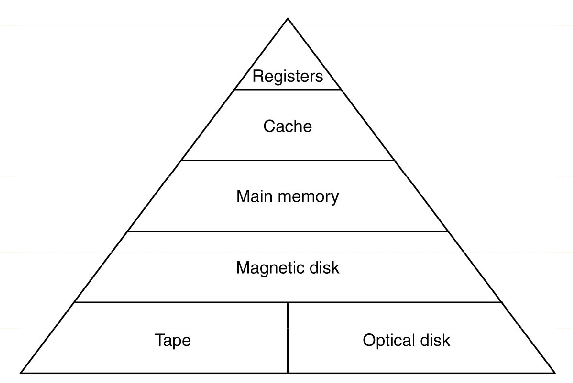
\includegraphics[scale=0.45]{../images/memory-h.png}
\label{memory-h}
\end{center}
\end{figure}
\subsubsection{Structure}
A word is an entity of bits that moves in and out of a memory unit as a group. 4-byte (32-bit) and 8-byte (64-bit) words are common in modern times. Each word in memory is associated with a single address. RAM is comprised of $k$ address lines which are responsible for selecting the source or target word within memory. There are $n$ data output lines which are responsible for the actual transfer of data. Lastly, there are control inputs, such as read/write indicators and chip selects, which identify which operations are currently being executed. When a RAM chip is executing a read cycle, it's read/write indicator is typically 0 (reading), it's chip select is 1 (use this chip). The RAM chip will at some point place data sourced from the location on the address lines on the data-bus using it's data lines. \newline\newline
Memory capacity is defined as $2^{k}$ words of $n$ bits in size. In a typical example, 16 gigabytes is the maximum addressable capacity With a 32-bit address bus. 
\subsubsection{Operations}
A write operation is used to transfer into memory a word that should be stored. It can be summarized as follows
\begin{itemize}
\item Apply the binary address of the desired memory location on the address bus.
\item Apply the binary data to be written to the data bus.
\item Activate the write input
\end{itemize}
A read operation is equivalent to the above except the write input is not activated and it is memory that is responsible for driving data on to the address bus. In the case where there are multiple memory chips in the architecture, a \textit{chip select} facilitates enabling and disabling of specific memory chips. Chip select logic is typically driven from the address lines to accomplish this. Each chip will then have it's own address space and (in this configuration) is \textbf{memory mapped.} Figure \ref{read-write} shows the cycles is much greater detail. Note how all operations in this diagram occur on a clock edge. Note particularly that it takes more than one of these clock cycles to complete a full read or write cycle. Lastly, note how the full length of the read write cycles are not necessarily the same. 

\begin{figure}
\caption{Timing Diagrams of the read write cycle\cite{LOGICDESIGN}}
\begin{center}
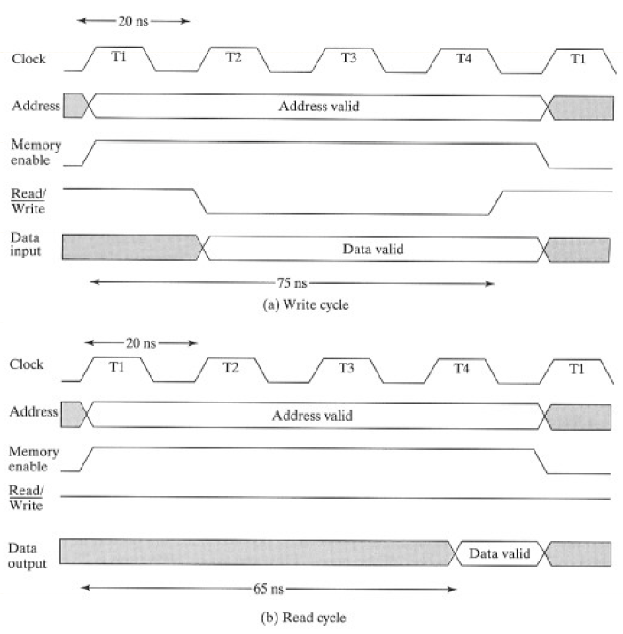
\includegraphics[scale=0.40]{../images/read-write-timing.png}
\label{read-write}
\end{center}
\end{figure}

When the CPU is executing a read or write cycle, especially in this configuration, it will be busy waiting around for the slower memory to complete it's operation. At this point the CPU cannot conduct any transformations. For this reason, computer systems will often contain levels of much faster memory of differing sizes. We will discuss later is this chapter some techniques that assist us in minimizing this overhead. \newline\newline
At the circuit level, RAM can be \textbf{static} or \textbf{dynamic}. Static RAM uses an array of SR Latches \cite{SRLATCH} coupled with selection logic. Dynamic RAM actually use capacitor arrays which require periodic refresh. Static RAM typically has shorter read/write cycles but consumes more power than DRAM due to the requirement for constant charge. Economically, DRAM is cheaper to produce in larger quantities. SRAM my typically be found in on-chip cache, whereas DRAM is more commonly found in main system memory. 
\subsection{Memory Addressing}
As mentioned earlier, the physical address space of a computer is defined by the width of it's address bus. Components of the system will each have their own physical address space, which will be a sub-set of the entire address space. It is the responsibility of the \textbf{memory management unit} or MMU, to manage the mapping of \textbf{virtual} to physical addresses. In effect, the MMU provides a means for a program executing on the CPU to not have to worry about exactly where in the address space a particular piece of memory is mapped. This is a very important concept that you will see repeated in various flavours when we look at how operating systems work. 
\newline\newline
An MMU will divide the physical address space into \textbf{pages} of typically 4Kb in size. When a program references a particular location in its \textit{virtual address space} the MMU will use some translation mechanism to map to a physical address location. The size of the page allows the MMU to map virtual to physical address spaces, while keeping it's internal map relatively small and helping to keep the address translation fast. We will talk about these in more detail in later articles. 
\section{Execution of Instructions}
An \textit{instruction} is a sequence of bits that tells the CPU to perform a particular operation. The core instruction contains bit configurations that manipulate the control and data-paths of the CPU. Instructions may also have \textbf{operands} which define meta-data related to the instruction. Such meta-data includes location of data to be operated on in memory, or the actual data itself. In essence, programs are sequences of these instructions executed in some order by the CPU.
\subsection{Instruction Sets}
The instruction set is the set of machine-language primitives that can be directly executed on a processor. Historically, programmers would write programs directly using this set. However, in recent times, almost all except very specialist programming is done in much higher level languages. These languages are translated into the machine language that more directly encodes these instructions. This will typically happen at several layers of indirection before actual machine code is produced. Therefore, modern processors provide instruction sets that are designed to be translated to by compilers, and often contain specialist instructions that assist compilers in writing efficient programs. Nevertheless, these instructions can typically be categorized as follows. 
\begin{itemize}
\item ALU Instructions - Add, Subtract, Multiply
\item Memory Instructions - Load and Storing of data
\item Control Instructions - Conditional Branch, Call, Return, Interrupt 
\item Specialized Instructions - FPU Extensions, MMX Instructions
\end{itemize}
The transition to less human readable instruction sets occurred in parallel with the rise in popularity of RISC CPUs. A \textbf{reduced instruction set} CPU, as the name suggests, contains a smaller set of instructions. Program optimization, therefore, at the compiler level. In contrast, a \textbf{complex instruction set} CPU contains more complex operations that will be optimized at the hardware level. There is on-going debate as to which approach is the most desirable approach. Processors of the x86 range take the CISC approach, while PowerPC and some ARM processors will take the RISC approach. See \cite{RISC-CISC} for a comprehensive discussion.
\section{Fetch, Decode and Execute Cycle}
A \textbf{register} is a temporary storage location inside the CPU. The \textbf{register file} of the CPU will contain several general purpose registers of varying classes. Data registers are designed to contain data that is being operated on. Address registers are designed to contain locations in memory. Special purpose registers compliment the above file. The \textbf{program counter} points to the location in memory of the instruction which is to be next executed. A \textbf{memory data register} is often used as a buffer to memory data as it moves between the CPU and memory. Lastly, the \textbf{instruction register} contains the instruction that has just been fetched from memory. The control unit will decode the operation contained in the instruction set, and if necessary fetch data, perform operations and store data back. 
\newline\newline
\subsection{Fetch}
This part of the cycle is responsible for retrieving the next instruction that is pointed to in memory by the PC by executing a read cycle, placing the instruction in the IR. The PC is incremented by 1 after this operation completes, however since some instructions can modify the PC - i.e. jumps or branches - this does not mean that this will be the PC location at the start of the next cycle.   
\subsection{Decode}
The control path decodes the instruction in the IR. This involves executing logic that will understand exactly what inputs to apply to the ALU, or which operation needs to be applied to the PC, or perhaps if we need to execute a new cycle. 
\subsection{Read Effective Address}
If an instruction is decoded and is found that an operand points to a location in memory where where data must be fetched from, then one or more read cycles is executed to fetch the operands in question. 
\subsection{Execute}
The execute phase is responsible for the actual data-transform operation that must take place. Part of the execute cycle includes write back of any results into memory if required. 
\newline\newline
Figure \ref{program} shows a subset of a program listing that multiplies some matrices together. It illustrates exactly how instructions in a program map to encodings in memory. To the left of the listing, it can be seen how the assembly language encoding is stored in memory, and eventually in the IR. As an exercise, use the MC68000 reference found at \cite{68KREF} to fully understand how this program is cross compiled and manipulates the ALU. See \cite{LYNCH-68K} for the full listing and some for some introductory understanding. Bonus marks for anybody who can improve this listing to be more concise - there are numerous possibilities. E-mail answers to me at the usual address. 
\begin{figure}
\caption{A MC68k Assembly Program Snippit \cite{LYNCH-68K}}
\begin{center}
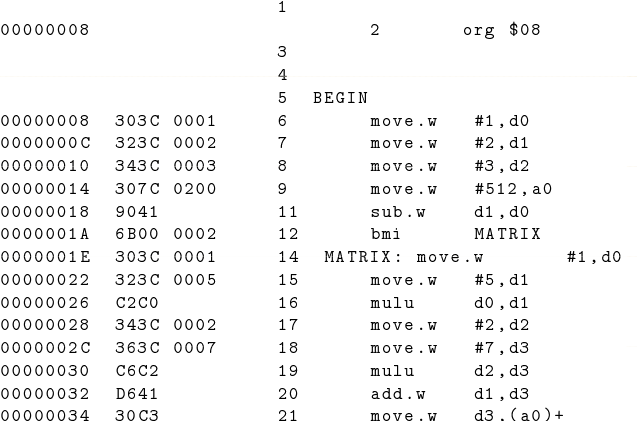
\includegraphics[scale=0.50]{../images/assembly-program.png}
\label{program}
\end{center}
\end{figure}
\section{Caches}
There is some possibility that you may never have to work at the level that we have worked at so far in this article. It is still a good exercise to understand the underlying machine, and in the coming years with particular importance placed on multi-core CPU's, some of the above information will come in handy. However, if there is one section of this article that you understand backwards, do extra reading on and put into practice, it should be this!\newline\newline 
Conceptually, a cache is a mechanism of storing data transparently, so that the cost of future retrievals of that same data is much less than the cost of the first retrieval. In essence, the average time to access this data is reduced. There are a multitude of applications of this concept in computer systems, from web caches to disk caches. Here, we will discuss caches as implemented at the CPU level. \newline\newline
A CPU cache is a layer of memory that sits between main memory and the CPU. It is much smaller than main system memory, but much faster. The aim of the CPU cache is to reduce the average time the CPU spends waiting on an memory access cycle to complete. Cache memory access times are much closer to the CPU clock period than standard memory access, resulting in a compression of the timing cycle length we see in \ref{read-write}.
\subsection{Locality of Reference}
The \textbf{principle of locality of reference} states that the collection of data locations referenced over a short period of time on a running computer often consists of well reproducible clusters.  More plainly, programs tend to access the same memory locations multiple times over the running time of the program. This is known as \textbf{temporal locality}. Also, if a specific location is referenced at any particular time, it is likely that a nearby memory location will be accessed before the completion of the program. This is known as \textbf{spacial locality.} We can take advantage of temporal locality, moving the contents of frequently accessed locations to the much faster, but smaller CPU cache memory. Similarly, we may move the contents of locations that are nearby to the most frequently accessed locations. 
\subsection{Structure of CPU Cache}
CPU cache memory is organised as a collection of \textbf{cache lines.} When full, each line has a copy of the contents of some location in memory. Each line also tracks the address of this location. Since we need to track whether the data is consistent with main memory, a \textbf{dirty bit} is also associated with this cache line. When a CPU addresses a location that is contained in cache memory, we call it a \textbf{cache hit}. Otherwise, we call it a \textbf{cache miss.} Depending on our cache management strategy a cache miss may result in a new cache line entry. Since the cache is of finite size and hugely smaller than main  memory, when each cache line is valid, we must choose to \textbf{evict} an existing line. This is done in accordance with our \textbf{replacement policy.}\newline\newline
This algorithm is likely concerned with predicting which cache entry is least likely to produce a cache hit in the future. A plethora of algorithms exist to do this, one of the simpler is a \textbf{least recently used} approach. A \textbf{write through} cache writes a store operation to memory every time, whereas a write back cache simply mark a line as dirty and write back to memory at some later stage. This is typically upon eviction. Since main memory is visible to numerous entities, not least other processors, caches can quickly become \textbf{stale} with respect to main memory and also to other caches within the system. \textbf{Cache coherence protocols} define the behaviour of concurrent reads and writes to the same memory location. This can be a very complex task, and is something which we will return to in detail in later articles. 
\subsection{Impact of Replacement Policy}
If the replacement policy enforcement algorithm is free to choose any location in the cache, it is termed a \textbf{fully associative} cache. If each memory location can exist in one location only it is known as a \textbf{directly mapped cache.} \textbf{N-Way associative caches} represent a middle ground. For example, a two way set associative cache defines two locations in the cache that each main memory location could possibly exist\newline\newline
Directly mapped cache return the fastest hit times, which associative caches have a relatively lower miss rate. Caches that use elements of both are constructed in an attempt to find a middle-ground between the extremes of both goals. Figure \ref{cache} illustrates this. 
\begin{figure}
\caption{Direct Mapped vs. Associative Cache \cite{CACHE}}
\begin{center}
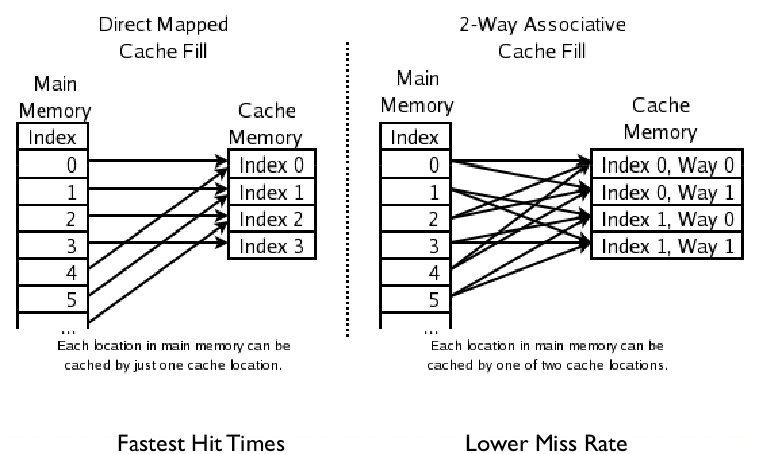
\includegraphics[scale=0.45]{../images/cache.png}
\label{cache}
\end{center}
\end{figure}
\bibliography{../biblio/techfundamentals.bib}{}
\bibliographystyle{plain}
\begin{center}
\end{center}
\end{document}
